\chapter{Modelo del Negocio}
\section{Contexto}
La Franquicia de Farmacias "Fran Farmacias" se dedica a la venta de medicamentos que requieren o no receta. La franquicia consta con un único dueño y múltiples empleados atendiendo las sucursales, de la misma manera el supervisor de la sucursal en la que esta asignado, verifica en la apertura y al cierre del turno que la operación de la sucursal sea de la mejor manera posible y lo mismo pasa en las diferentes sucursales de la franquicia\\

\section{Términos del Negocio}

Cliente: Se refiere a todas las personas físicas y morales que Compran medicamentos ya sea que estos sean clientes registrados en el sistema o sin registrar.\\

Cliente Preferente: Se refiere a todas aquellas personas físicas y morales que Compran medicamentos y que están registrados en el sistema, estos clientes cuentan con un monedero electrónico


Dosis: Cantidad a ingerir o suministrar expresado en unidades de volumen o peso(gramos) por unidad de un Medicamento.\\

Dueño: Es propietario de la farmacia y de todas sus sucursales, se encarga de la contratación de todos los Empleados, es el Empleado con mayor rango en “Fran Farmacias”.\\

Empleado: Se refiere a cualquier persona que labore en la empresa exceptuando al Dueño.\\

Estado: Hace referencia a los elementos, definiendo un elemento como: Cliente, Sucursal, Medicamento, Empleado, Paquete de descuento y Proveedor, Donde dicho elemento puede ser manipulado en operaciones de lectura y escritura (Estado activado) o solo lectura(Estado desactivado)\\

Ingrediente Activo: Sustancia del Medicamento con composición química exactamente conocida y que es capaz de producir efectos o cambios sobre el cuerpo de quien lo consume.\\

Laboratorio Farmacéutico: Aquellas personas físicas o jurídicas que, previamente autorizadas por la Administración competente, fabriquen de forma industrial Medicamentos o participen en alguna de sus fases.\\

Lote: Es una clave de identificación de los Medicamentos de un mismo proceso de fabricación.Tiene valor para el Laboratorio Farmacéutico. Consta de una letra , que indica el año de fabricación, y de un número.\\

Medicamento: Producto que sirve para curar, prevenir una enfermedad, para reducir sus efectos sobre el organismo o para aliviar un dolor físico.\\

Monedero electrónico: Dinero abonado por una devolución a la cuenta del cliente preferente.\\

Paquete De Descuento: Son paquetes que añade el dueño cuando se esta por caducar un medicamento, o es temporada en la que un medicamento tiene un rango de venta mayor que otros y se aprovecha para hacer un descuento de esos medicamentos, al conjunto de medicamentos que se van a poner en descuento es un: paquete de Descuento.\\

Presentación Del Medicamento: Es el tipo de Presentación del medicamento, los cuales son:\\
1.-Presentación Solida: Polvos, Cápsulas, Tabletas o Comprimidos, Píldoras, Grageas, Supositorios, Óvulos\\
2.-Presentaciones Semisolidas: Pomadas o Cremas\\
3.-Presentaciones Liquidas: Soluciones, Jarabes, Colirios, Lociones, Linimentos, Elixir, Enemas, Inhalaciones, Aerosoles\\

Sucursal: Una extensión de la farmacia donde se opera como la farmacia original.
Esta Sucursal tiene nombre Único \\

Supervisor: (es un tipo de Empleado) Es un empleado con mayor Jerarquía que Empleado pero menor que Dueño.\\

Venta: Son los datos que se guardan de una venta de medicamento realizada.\\

Vía de Administración:  Es la forma en la que el cliente se tiene que aplicar el medicamento.entre estas están: Vía Digestiva, Vía Oral, Vía Sublingual, Gastroenteritis, Vía Rectal, Vía Parental, Vía Respiratoria, Vía Tópica, Vía Oftálmica, Vía Ótica, Vía Transdérmica.\\
\newpage
\section{Modelo de Dominio del problema}

	El modelo del dominio del problema se muestra en la figura~\ref{fig:modeloDeDominio}, a continuación se describen cada una de las entidades y sus relaciones.
	
\begin{figure}[htbp!]
	\begin{center}
		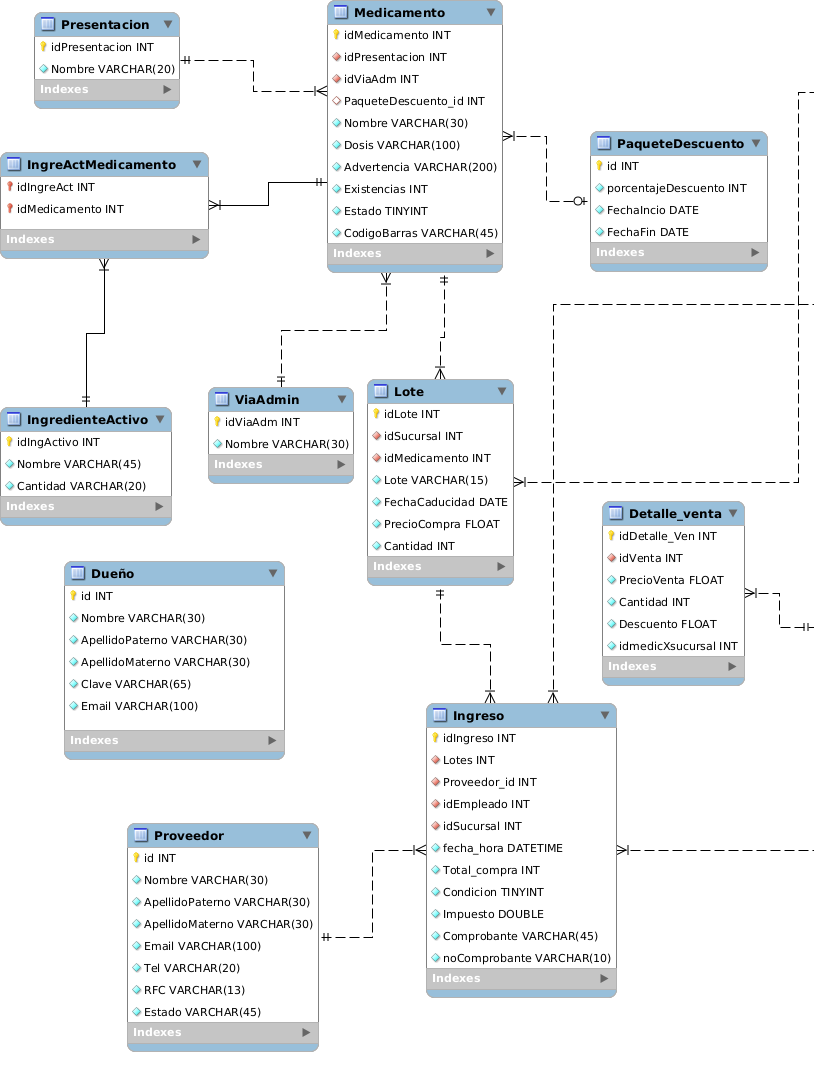
\includegraphics[width=.9\textwidth]{images/diagramaRelacional1}
		\caption{Modelo del dominio del problema}
		\label{fig:modeloDeDominio}
	\end{center}
\end{figure}

\begin{figure}[htbp!]
	\begin{center}
		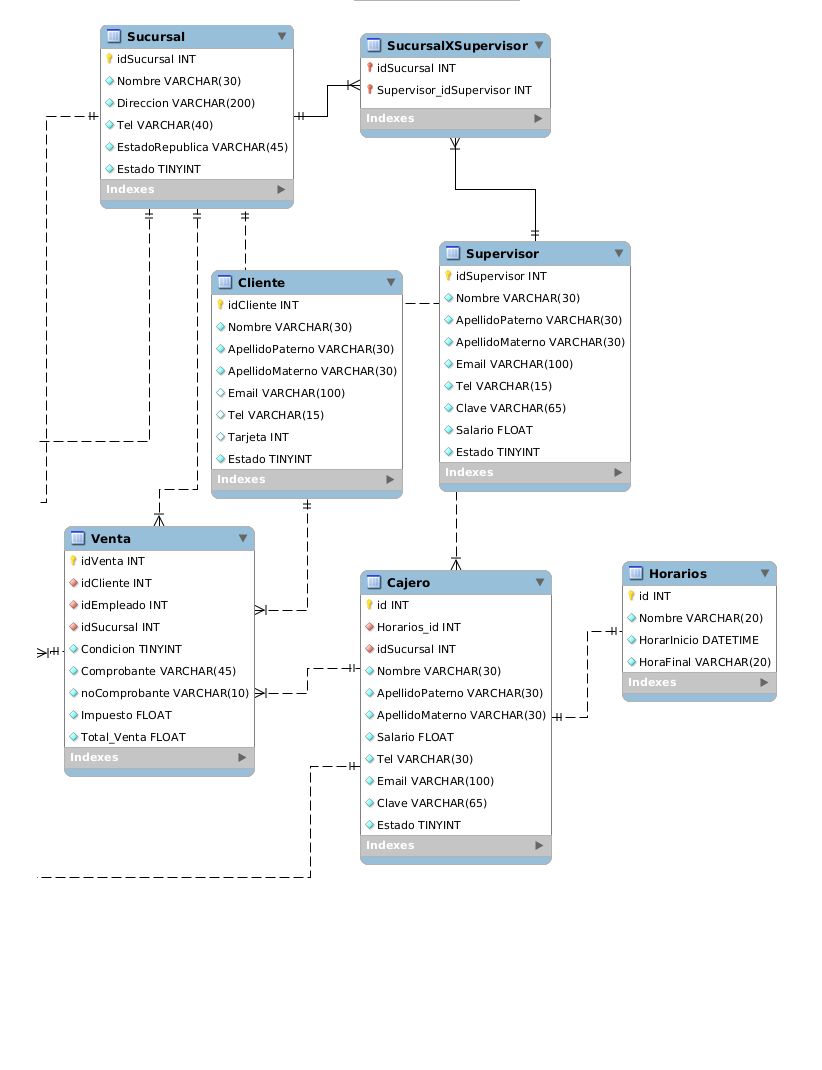
\includegraphics[width=.9\textwidth]{images/diagramaRelacional2}
		\caption{Modelo del dominio del problema}
		\label{fig:modeloDeDominio}
	\end{center}
\end{figure}
\newpage
%---------------------detalle de las entidades

%- - - - - - - - - - - - - - - - - - - - - - - - - - - - - 
\newenvironment{cdtEntidad}[2]{%
	\def \varBusinessEntityId{#2}%
	\hypertarget{#1}{\hspace{1pt}}%
	\newline%
	\noindent{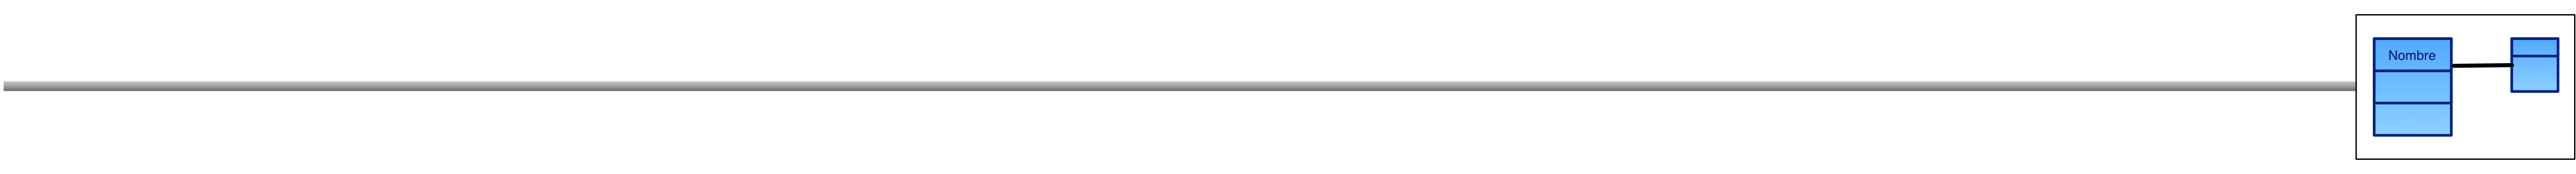
\includegraphics[width=\textwidth]{images/uc/classRule}}%
	\vspace{-25pt}%
	\subsection{Entidad: #2}%
	\noindent\begin{longtable}{|p{.2\textwidth}| p{.15\textwidth} | p{.46\textwidth} |p{.08\textwidth} |}%
	\hline%
	\multicolumn{4}{|c|}{{\cellcolor{colorSecundario}\color{white}Atributos}}\\ \hline%
	{\cellcolor{colorAgua}Nombre} &%
	{\cellcolor{colorAgua}Tipo} &%
	{\cellcolor{colorAgua}Descripción} &%
	{\cellcolor{colorAgua}Requerido}%
	\\ \hline%
	\endhead%
}{%
	\end{longtable}%
}

\newcommand{\brAttr}[5]{%
	{\bf\hypertarget{\varBusinessEntityId:#1}{#2}} & {\em{#3}} & {#4} & #5 \\\hline
}

\newcommand{\cdtEntityRelSection}{%
	\multicolumn{4}{|c|}{{\cellcolor{colorSecundario}\color{white}Relaciones}}\\ \hline%
	{\cellcolor{colorAgua}Tipo de relación} &%
	{\cellcolor{colorAgua}Entidad} &%
	\multicolumn{2}{|c|}{{\cellcolor{colorAgua}Rol}}
	\\ \hline%
}

\newcommand{\brRelComposition}{{\color{colorPrincipal}$\Diamondblack$\hspace{-1pt}---Composición}}
\newcommand{\brRelAgregation}{{\color{colorPrincipal}$\Diamond$\hspace{-1pt}---Agregación}}
\newcommand{\brRelGeneralization}{{\color{colorPrincipal}$\lhd$\hspace{-1pt}---Generalización}}

\newcommand{\brRel}[3]{%
	{\em{#1}} & {\bf{#2}} & \multicolumn{2}{|l|}{#3}\\\hline
}
\newpage


%- - - - - -------------------------------------------------
\begin{cdtEntidad}{Dueño}{Dueño}
\brAttr{ID}{ID}{int}{Número de registro utilizado para identificar al Dueño}{Sí}
	\brAttr{nombre}{Nombre}{String}
		{Nombre o nombres del Dueño.}{Sí}
		
	\brAttr{ApellidoPaterno}{Apellido Paterno}{String}
		{Apellido Paterno del Dueño.}{Sí}
		
	\brAttr{ApellidoMaterno}{ApellidoMaterno}{String}
		{Apellido Materno del Dueño.}{No}
		
	\brAttr{Email}{Email}{String}
		{Correo del Dueño para enviar información Laboral y entrar al sistema junto con su Clave.}{Sí}
		
	\brAttr{Clave}{Clave}{String}
		{Forma de permitir al Dueño ingresar en el sistema junto con su correo.}{Sí}
		
\end{cdtEntidad}

%- - - - - -------------------------------------------------
\begin{cdtEntidad}{Supervisor}{Supervisor}
\brAttr{registro}{Registro}{int}{Número de registro utilizado para identificar al supervisor}{Sí}
	\brAttr{nombre}{Nombre}{String}
		{Nombre o nombres del Supervisor.}{Sí}
		
	\brAttr{primerApellido}{Primer apellido}{String}
		{Apellido Paterno del Supervisor.}{Sí}
		
	\brAttr{segundoApellido}{Segundo apellido}{String}
		{Apellido Materno del Supervisor.}{No}
		
	\brAttr{Email}{Email}{String}
		{Correo del Empleado para enviar información Laboral y identificar al Supervisor en el sistema con sus respectivos permisos.}{Sí}

	\brAttr{telefono}{Teléfono}{int}
		{Teléfono para contactar al Supervisor.}{Sí}
		
	\brAttr{Contraseña}{Contraseña}{String}
		{Forma de permitir al Supervisor ingresar en el sistema junto con su correo.}{Sí}
		
	\brAttr{Estado}{Estado}{TINYINT}
		{Estado del supervisor, puede estar activado o desactivado (un tipo de dato TINYINT representa un carácter , por razones de eficiencia se utiliza este tipo de dato en vez de un booleano).}{Sí}	
	
	\brAttr{Sucursal}{Sucursal}{Sucursal}
		{Sucursal de la que esta a cargo el supervisor.}{Sí}

		\cdtEntityRelSection
	\brRel{\brRelAgregation}{Sucursal}{Muchos Supervisores trabajan en muchas Sucursales}
\end{cdtEntidad}



%- - - - - -------------------------------------------------
\begin{cdtEntidad}{Cajero}{Cajero}
\brAttr{ID}{ID}{int}{Número de registro utilizado para identificar al Cajero}{Sí}
	\brAttr{nombre}{Nombre}{String}
		{Nombre o nombres del Cajero.}{Sí}
		
	\brAttr{ApellidoPaterno}{Apellido Paterno}{String}
		{Apellido Paterno del Cajero.}{Sí}
		
	\brAttr{ApellidoMaterno}{ApellidoMaterno}{String}
		{Apellido Materno del Cajero.}{No}
		
	\brAttr{Salaro}{Salariol}{Float}
		{Salario a que cobra el cajero.}{Sí}
		
	\brAttr{telefono}{Teléfono}{String}
		{Teléfono para contactar al Cajero.}{Sí}
		
	\brAttr{Email}{Email}{String}
		{Correo del Cajero para enviar información Laboral y entrar al sistema junto con su Clave.}{Sí}
		
	\brAttr{Clave}{Clave}{String}
		{Forma de permitir al Cajero ingresar en el sistema junto con su correo.}{Sí}
	
	\brAttr{Estado}{Estado}{TINYINT}
		{Estado del cajero, puede estar activado o desactivado (un tipo de dato TINYINT representa un carácter , por razones de eficiencia se utiliza este tipo de dato en vez de un booleano).}{Sí}	
	
	\brAttr{Sucursal}{Sucursal}{Sucursal}
		{Sucursal de la que esta a cargo el supervisor.}{Sí}

		\cdtEntityRelSection
	\brRel{\brRelAgregation}{Horario}{El Cajero tiene un horario}
	\brRel{\brRelAgregation}{Cliente}{Un Cajero atiende a muchos clientes}
	\brRel{\brRelAgregation}{Venta}{Un Cajero realiza muchas ventas}
	\brRel{\brRelComposition}{Sucursal}{Una sucursal se compone de muchos cajeros}
\end{cdtEntidad}

%- - - - - - - - - - - - - - - - - - - - - - - - - - - - - 
\begin{cdtEntidad}{Cliente}{Cliente}
	\brAttr{ID}{ID}{int}{Número de registro utilizado para identificar al Cliente}{Sí}
	\brAttr{nombre}{Nombre}{String}
		{Nombre o nombres del Cliente.}{Sí}
		
	\brAttr{ApellidoPaterno}{Apellido Paterno}{String}
		{Apellido Paterno del Cliente.}{Sí}
		
	\brAttr{ApellidoMaterno}{ApellidoMaterno}{String}
		{Apellido Materno del Cliente.}{No}
		
	\brAttr{Email}{Email}{String}
		{Correo del cliente para enviar información sobre promociones.}{Sí}
		
	\brAttr{telefono}{Teléfono}{String}
		{Teléfono para contactar al Cliente.}{Sí}
		
	\brAttr{Tarjeta}{Tarjeta}{int}
		{forma única de hacer devoluciones sobre compras hechas a los clientes.}{si}

	\brAttr{Estado}{Estado}{TINYINT}
		{Estado del Cliente, puede estar activado o desactivado (un tipo de dato TINYINT representa un carácter , por razones de eficiencia se utiliza este tipo de dato en vez de un booleano).}{Sí}	
		
		\cdtEntityRelSection
	\brRel{\brRelAgregation}{Cliente}{El Cliente Compra en Sucursal}
\end{cdtEntidad}
%---------------------------------------------------------

\begin{cdtEntidad}{Medicamento}{Medicamento}
	\brAttr{ID}{ID}{Int}{Identificador del Medicamento.}{Sí}
	
	\brAttr{IDViaAdministracion}{IDViaAdministracion}{Int}{Identificador de la vía de Administración del Medicamento.}{Sí}
	
	\brAttr{IDPaqueteDescuento}{IDPaqueteDescuento}{Int}{Identificador del paquete de descuento al que pertenece el Medicamento.}{Sí}

	\brAttr{IDPresentacion}{IDPresentaicon}{Int}{Identificador del tipo de presentación del Medicamento.}{Sí}
	
	\brAttr{Nombre}{Nombre}{String}{Nombre del Medicamento.}{Sí}
	
	\brAttr{Marca}{Marca}{String}{Marca del medicamento}{Sí}
	
	\brAttr{FechaCaducidad}{FechaCaducidad}{DATE}{La fecha de caducidad del medicamento}{si}
	
	\brAttr{Lote}{Lote}{Int}{el numero de lote del medicamento}{Sí}
	
	\brAttr{ViaDeAdministracion}{ViaDeAdministracion}{String}
		{Indica la forma en la que el medicamento debe ser ingerido}{si}
		
	\brAttr{Advertencias}{Advertencias}{string}
		{Las precauciones que se deben tomar en cuenta con el medicamento}{si}
		
	\brAttr{PrecioPublico}{PrecioPublico}{int}
		{El precio al que se le vende al cliente.}{si}
		
	\brAttr{PrecioCompra}{PrecioCompra}{Int}
		{El precio al que se compra el medicamento al proveedor}{si}
		
	\brAttr{noIngedientesActivos}{noIngredientesActivos}{int}
		{número de ingredientes activos que contiene el medicamento}{si}

		\cdtEntityRelSection
	\brRel{\brRelComposition}{Medicamento}{El Medicamento Esta compuesto por IngredienteActivo}
	\brRel{\brRelComposition}{Medicamento}{El Medicamento tiene una Presentacion}
	\brRel{\brRelComposition}{Medicamento}{El Medicamento tiene una viaAdministracion}
	\brRel{\brRelComposition}{Medicamento}{El Medicamento tiene un Lote}
	\brRel{\brRelAgregation}{Medicamento}{El Medicamento se agrega a un paquete de descuento}
\end{cdtEntidad}
%- - - - - - - - - - - - - - - - - - - - - - - - - - - - - 
\begin{cdtEntidad}{IngredienteActivo}{IngredienteActivo}
	\brAttr{ID}{ID}{Int}
		{El identificador al que pertenece el ingrediente activo}{Sí}
	\brAttr{Nombre}{Nombre}{String}
		{El Nombre del ingrediente activo}{Sí}
	\brAttr{Cantidad}{Cantidad}{String}
		{La cantidad del ingrediente activo presente en el Medicamento}{Sí}

\end{cdtEntidad}
%---------------------------------------------------------

%- - - - - - - - - - - - - - - - - - - - - - - - - - - - - 
\begin{cdtEntidad}{Presentación}{Presentación}
	\brAttr{ID}{ID}{Int}
		{El identificador al que pertenece la Presentación Del Medicamento}{Sí}
	\brAttr{Nombre}{Nombre}{String}
		{El Nombre del tipo de presentación}{Sí}

\end{cdtEntidad}

%- - - - - - - - - - - - - - - - - - - - - - - - - - - - - 
\begin{cdtEntidad}{ViaAdministracion}{ViaAdministracion}
	\brAttr{ID}{ID}{Int}
		{El identificador al que pertenece a la Vía de Administración}{Sí}
	\brAttr{Nombre}{Nombre}{String}
		{El Nombre del tipo de Vía de Administración}{Sí}

\end{cdtEntidad}

%- - - - - - - - - - - - - - - - - - - - - - - - - - - - - 
\begin{cdtEntidad}{Lote}{Lote}
	\brAttr{ID}{ID}{Int}
		{El identificador al que pertenece el Lote}{Sí}
	\brAttr{Nombre}{Nombre}{String}
		{El Nombre compuesto del lote}{Sí}
	\brAttr{FechaCaducidad}{FechaCaducidad}{DATE}
		{Fecha en la que el medicamento caduca}{Sí}
	\brAttr{PrecioCompra}{PrecioCompra}{DATE}
		{Precio en el que se compro el Lote de medicamento}{Sí}
	\brAttr{Cantidad}{Cantidad}{DATE}
		{Cantidad de medicamento que se registro por lote}{Sí}
\end{cdtEntidad}

%------------------------------------------------------------
\begin{cdtEntidad}{PaqueteDescuento}{PaqueteDescuento}
	\brAttr{ID}{ID}{Int}
		{Identificador del descuento.}{Sí}
	\brAttr{porcentajeDescuento}{porcentajeDescuento}{Int}
		{Descuento de porcentaje(\%) a aplicar sobre los medicamentos}{si}
	\brAttr{FechaInicio}{FechaInicio}{DATE}
		{La fecha en la que se empieza a aplicar el descuento}{si}
	\brAttr{FechaFin}{FechaFin}{DATE}
		{Fecha limite para aplicar Descuento}{Sí}
\end{cdtEntidad}

%- - - - - - - - - - - - - - - - - - - - - - - - - - - - - 
\begin{cdtEntidad}{Venta}{Venta}

	\brAttr{idVenta}{idVenta}{int}
		{Identificador del la venta}{si}
		
	\brAttr{IDCliente}{IDCliente}{Int}
		{Cliente al que se le vendió si es que este esta registrado en el sistema.}{si}
		
	\brAttr{IDSucursal}{IDSucursal}{Int}
		{Sucursal en la que se realizó la venta}{si}
		
	\brAttr{IDEmpleado}{IDEmpleado}{Int}
		{Empleado que realizó la venta}{si}
		
	\brAttr{Condición}{Condición}{TINYINT}
		{Estado de la venta, puede estar activa o cancelada (un tipo de dato TINYINT representa un carácter , por razones de eficiencia se utiliza este tipo de dato en vez de un booleano).}{Sí}	

	\brAttr{Comprobante}{Comprobante}{String}
		{Comprobante de la venta}{si}
		
	\brAttr{noComprobante}{noComprobante}{String}
		{Identificador de Comprobante de la venta}{si}
		
	\brAttr{Impuesto}{Impuesto}{Float}
		{Impuesto de la venta}{si}
		
	\brAttr{TotalVenta}{TotalVenta}{Float}
		{Costo total de la venta realizada}{si}
		
		\cdtEntityRelSection
		
	\brRel{\brRelComposition}{DetalleVenta}{Una Venta tiene muchos detalles de venta}
	
\end{cdtEntidad}
%- - - - - - - - - - - - - - - - - - - - - - - - - - - - - 

%- - - - - - - - - - - - - - - - - - - - - - - - - - - - - 
\begin{cdtEntidad}{DetalleVenta}{DetalleVenta}

	\brAttr{idDetalleVen}{idDetalleVen}{int}
		{Identificador del Detalle de la venta}{si}
		
	\brAttr{IDVenta}{IDVenta}{Int}
		{Identificador de la Venta}{si}
		
	\brAttr{PrecioVenta}{PrecioVenta}{Int}
		{Precio de la venta realizada}{si}
		
	\brAttr{Cantidad}{Cantidad}{Int}
		{Cantidad por la cual se realizó la venta}{si}
		
	\brAttr{Descuento}{Descuento}{Float}
		{Descuento aplicado sobre la venta.}{Sí}	
	
\end{cdtEntidad}
%- - - - - - - - - - - - - - - - - - - - - - - - - - - - - 

%- - - - - -------------------------------------------------
\begin{cdtEntidad}{Proveedor}{Proveedor}
\brAttr{ID}{ID}{int}{Número de registro utilizado para identificar al proveedor}{Sí}
	\brAttr{nombre}{Nombre}{String}
		{Nombre o nombres del proveedor.}{Sí}
		
	\brAttr{ApellidoPaterno}{Apellido Paterno}{String}
		{Apellido Paterno del proveedor.}{Sí}
		
	\brAttr{ApellidoMaterno}{ApellidoMaterno}{String}
		{Apellido Materno del proveedor.}{No}

	\brAttr{Email}{Email}{String}
		{Correo del proveedor para poder contactar con el.}{Sí}
		
	\brAttr{telefono}{Teléfono}{String}
		{Teléfono para contactar al proveedor.}{Sí}
		
	\brAttr{RFC}{RFC}{String}
		{RFC del proveedor.}{Sí}
	
	\brAttr{Estado}{Estado}{TINYINT}
		{Estado del proveedor, puede estar activado o desactivado (un tipo de dato TINYINT representa un carácter , por razones de eficiencia se utiliza este tipo de dato en vez de un booleano).}{Sí}	
\end{cdtEntidad}

%- - - - - - - - - - - - - - - - - - - - - - - - - - - - - 

\begin{cdtEntidad}{Ingreso}{Ingreso}
\brAttr{ID}{ID}{int}{Número de registro utilizado para identificar el ingreso}{Sí}
	\brAttr{FechaHora}{FechaHora}{DATETIME}
		{Fecha y Hora del ingreso.}{Sí}
		
	\brAttr{TotalCompra}{TotalCompra}{Int}
		{Cantidad total de la compra a ingresar.}{Sí}
		
	\brAttr{Condición}{Condición}{TINYINT}
		{Condición de la compra a ingresar.}{No}

	\brAttr{Impuesto}{Impuesto}{Double}
		{Impuesto Aplicado sobre la compra a ingresar.}{Sí}
		
	\brAttr{Comprobante}{Comprobante}{String}
		{Comprobante de la compra realizada.}{Sí}
		
	\brAttr{RFC}{RFC}{String}
		{RFC del proveedor.}{Sí}
	
	\brAttr{Estado}{Estado}{TINYINT}
		{Estado del proveedor, puede estar activado o desactivado (un tipo de dato TINYINT representa un carácter , por razones de eficiencia se utiliza este tipo de dato en vez de un booleano).}{Sí}	
		
		\cdtEntityRelSection
	\brRel{\brRelComposition}{Lote}{El Ingreso tiene un Lote}
	\brRel{\brRelComposition}{Proveedor}{El Ingreso tiene muchos proveedores}
	\brRel{\brRelComposition}{Proveedor}{El Ingreso tiene muchos proveedores}
	\brRel{\brRelComposition}{Cajero}{El Ingreso lo registra un cajero}
	\brRel{\brRelComposition}{Sucursal}{El Ingreso se realiza en una Sucursal}
\end{cdtEntidad}








%- - - - - - - - - - - - - - - - - - - - - - - - - - - - - 
\begin{cdtEntidad}{Sucursal}{Sucursal}

	\brAttr{idSucursal}{idSucursal}{Int}
		{Identificador único de la sucursal}{Sí}
		
	\brAttr{Nombre}{Nombre}{String}
		{Nombre de la sucursal.}{Sí}

	\brAttr{Dirección}{Dirección}{String}
		{Localización de la sucursal.}{Sí}
	
	\brAttr{Teléfono}{Teléfono}{String}
		{Teléfono de contacto de la sucursal.}{Sí}
		
	\brAttr{EstadoRepublica}{EstadoRepublica}{String}
		{Estado de la República donde esta ubicada la sucursal.}{Sí}
		
	\brAttr{noComprobante}{noComprobante}{String}
		{Identificador del Comprobante sobre la compra realizada.}{Sí}	
\cdtEntityRelSection
	\brRel{\brRelComposition}{Lote}{La sucursal tiene muchos Ingresos de medicamentos}
	\brRel{\brRelComposition}{Lote}{La sucursal tiene muchas ventas de medicamentos}

\end{cdtEntidad}
%- - - - - - - - - - - - - - - - - - - - - - - - - - - - - 

\begin{cdtEntidad}{Horarios}{Horarios}

	\brAttr{ID}{ID}{Int}
		{Identificador único del Horario}{Sí}
		
	\brAttr{Nombre}{Nombre}{String}
		{Nombre del Horario.}{Sí}

	\brAttr{HoraInicio}{HoraInicio}{DATETIME}
		{Hora de Inicio del Turno.}{Sí}
	
	\brAttr{HoraFinal}{HoraFinal}{DATETIME}
		{Hora de Fin del Turno.}{Sí}
		
\end{cdtEntidad}
%- - - - - - - - - - - - - - - - - - - - - - - - - - - - - 




%------------------------------------------------------
\newpage
\section{Reglas del Negocio}
%-----------------------------------------------------------------------------------------
\begin{BussinesRule}{BR1}{Desactivar Estado del empleado.}
	\BRitem[Tipo:] Regla de Autorización. 
	\BRitem[Clase:] Habilitadora. 
	\BRitem[Nivel:] Control. % Otras opciones para nivel: Control, Influencia.
	\BRitem[Descripción:] Si el empleado renuncia al trabajo O decide no renovar su contrato con nosotros simplemente se le desactivara su cuenta, así podemos checar todas las operaciones que este Empleado reviso durante su estadía en la sucursal o sucursales que operaba
	\BRitem[Motivación:] Evitar el acceso a todas las personas que no están registradas en el sistema o que no tienen un estado activado 
	\BRitem[Ejemplo positivo:]
	\BRitem[Ejemplo negativo:] 
\end{BussinesRule}

%-----------------------------------------------------------------------------------------
\begin{BussinesRule}{BR2}{Caducidad del Medicamento.}
	\BRitem[Tipo:] Regla de condición. 
	\BRitem[Clase:] Cronometrada. 
	\BRitem[Nivel:] Control. % Otras opciones para nivel: Control, Influencia.
	\BRitem[Descripción:] Un medicamento esta caduco cuando la fecha del medicamento es menor que la fecha actual
	\BRitem[Motivación:] Evitar venta de medicamento caducado
	\BRitem[Ejemplo positivo:] CaducidadMedicamento<FechaActual
	\BRitem[Ejemplo negativo:]  CaducidadMedicamento>FechaActual
\end{BussinesRule}
%-----------------------------------------------------------------------------------------
\begin{BussinesRule}{BR3}{Reporte Mensual de Mes.}
	\BRitem[Tipo:] Cronometrada. 
	\BRitem[Clase:] Condicional. 
	\BRitem[Nivel:] Control. % Otras opciones para nivel: Control, Influencia.
	\BRitem[Descripción:] La fecha limite para Presentar el reporte de venta mensual de la sucursal sera los Dias 28 de cada Mes.
	\BRitem[Motivación:]  Control Económico de la sucursal rápido y eficaz.
	\BRitem[Ejemplo positivo:]
	\BRitem[Ejemplo negativo:] 
\end{BussinesRule}
%-----------------------------------------------------------------------------------------
\begin{BussinesRule}{BR4}{Cancelar una Venta.}
	\BRitem[Tipo:] Habilitador. 
	\BRitem[Clase:] Autorización. 
	\BRitem[Nivel:] Control. % Otras opciones para nivel: Control, Influencia.
	\BRitem[Descripción:] En dado caso de que el cliente cancele su compra, el Supervisor debe de cancelar la operación de venta.
	\BRitem[Motivación:]  Control sobre las acciones que puede realizar cada empleado
	\BRitem[Ejemplo positivo:]
	\BRitem[Ejemplo negativo:] 
\end{BussinesRule}
%-----------------------------------------------------------------------------------------
\begin{BussinesRule}{BR5}{Cancelar una Venta.}
	\BRitem[Tipo:] Habilitador. 
	\BRitem[Clase:] Autorización. 
	\BRitem[Nivel:] Control. % Otras opciones para nivel: Control, Influencia.
	\BRitem[Descripción:] En dado caso de que el cliente cancele su compra, el Supervisor debe de cancelar la operación de venta.
	\BRitem[Motivación:]  Control sobre las acciones que puede realizar cada empleado
	\BRitem[Ejemplo positivo:]
	\BRitem[Ejemplo negativo:] 
\end{BussinesRule}
%-----------------------------------------------------------------------------------------
\begin{BussinesRule}{BR6}{Cantidad Máxima de venta a mostrador.}
	\BRitem[Tipo:] Habilitador. 
	\BRitem[Clase:] Integridad Referencial. 
	\BRitem[Nivel:] Cronometrada. % Otras opciones para nivel: Control, Influencia.
	\BRitem[Descripción:] La cantidad de medicamentos máxima que el cajero puede realizar es de 20
	\BRitem[Motivación:]  Control sobre las acciones que puede realizar cada empleado
	\BRitem[Ejemplo positivo:]   Venta Al Mostrador<20.
	\BRitem[Ejemplo negativo:] Venta al Mostrador>20.
\end{BussinesRule}
%-----------------------------------------------------------------------------------------
\begin{BussinesRule}{BR7}{Cantidad Excedente de venta a mostrador.}
	\BRitem[Tipo:] Habilitador. 
	\BRitem[Clase:] Integridad Referencial. 
	\BRitem[Nivel:] Ejecutiva. % Otras opciones para nivel: Control, Influencia.
	\BRitem[Descripción:] Si la cantidad a vender excede la cantidad de 20 , esta requiere autorización por parte del supervisor
	\BRitem[Motivación:]  Control sobre las acciones que puede realizar cada empleado
	\BRitem[Ejemplo positivo:]   Venta Al Mostrador>20.
	\BRitem[Ejemplo negativo:] Venta al Mostrador<20.
\end{BussinesRule}
%-------------------------------------------------------------------------------------------
\begin{BussinesRule}{BR8}{Compra del Medicamento.}
	\BRitem[Tipo:] Regla de condición. 
	\BRitem[Clase:] Cronometrada. 
	\BRitem[Nivel:] Control. % Otras opciones para nivel: Control, Influencia.
	\BRitem[Descripción:] Los medicamentos que compramos  a nuestros proveedores deben de tener una fecha de caducidad mayor a 2 años
	\BRitem[Motivación:] Evitar venta de medicamento caducado
	\BRitem[Ejemplo positivo:] CaducidadMedicamento>FechaActual
	\BRitem[Ejemplo negativo:]  CaducidadMedicamento<FechaActual
\end{BussinesRule}
%-----------------------------------------------------------------------------------------
%-------------------------------------------------------------------------------------------
\begin{BussinesRule}{BR9}{Sucursales operadas por el supervisor.}
	\BRitem[Tipo:] Regla de condición. 
	\BRitem[Clase:] Cronometrada. 
	\BRitem[Nivel:] Control. % Otras opciones para nivel: Control, Influencia.
	\BRitem[Descripción:] El supervisor puede tener un máximo de 3 sucursales bajo su supervisión y debe de tener un mínimo de 1 sucursal.  Y una sucursal puede tener un máximo de 3 supervisores y debe de tener mínimo 1 supervisor
	\BRitem[Motivación:] Sacar el máximo provecho de las operaciones diarias de las sucursales 
	\BRitem[Ejemplo positivo:]
	\BRitem[Ejemplo negativo:]  
\end{BussinesRule}
%-----------------------------------------------------------------------------------------
\begin{BussinesRule}{BR10}{Sucursales operadas por el cajero.}
	\BRitem[Tipo:] Regla de condición. 
	\BRitem[Clase:] Cronometrada. 
	\BRitem[Nivel:] Control. % Otras opciones para nivel: Control, Influencia.
	\BRitem[Descripción:] Una sucursal debe de tener un mínimo de 1 cajero por cada turno, hasta un máximo de 2 cajeros por cada turno
	\BRitem[Motivación:] Sacar el máximo provecho de las operaciones diarias de las sucursales 
	\BRitem[Ejemplo positivo:]
	\BRitem[Ejemplo negativo:]  
\end{BussinesRule}
%-----------------------------------------------------------------------------------------

\begin{BussinesRule}{BR11}{Jornadas Laborales.}
	\BRitem[Tipo:] Regla de condición. 
	\BRitem[Clase:] Cronometrada. 
	\BRitem[Nivel:] Control. % Otras opciones para nivel: Control, Influencia.
	\BRitem[Descripción:] La jornada Laboral de cada turno sera no mayor a 8 horas, entendiéndose que tenemos 3 turnos laborales; Turno Matutino 6:00 ->14:00; Turno Vespertino 14:00->22:00; Turno Nocturno 22:00->6:00
	\BRitem[Motivación:] Sacar el máximo provecho de las operaciones diarias de las sucursales 
	\BRitem[Ejemplo positivo:]
	\BRitem[Ejemplo negativo:]  
\end{BussinesRule}
%-----------------------------------------------------------------------------------------


\begin{BussinesRule}{BR11}{Jornadas Laborales.}
	\BRitem[Tipo:] Regla de condición. 
	\BRitem[Clase:] Cronometrada. 
	\BRitem[Nivel:] Control. % Otras opciones para nivel: Control, Influencia.
	\BRitem[Descripción:] La jornada Laboral de cada turno sera no mayor a 8 horas, entendiéndose que tenemos 3 turnos laborales; Turno Matutino 6:00 ->14:00; Turno Vespertino 14:00->22:00; Turno Nocturno 22:00->6:00
	\BRitem[Motivación:] Sacar el máximo provecho de las operaciones diarias de las sucursales 
	\BRitem[Ejemplo positivo:]
	\BRitem[Ejemplo negativo:]  
\end{BussinesRule}
%-----------------------------------------------------------------------------------------


\begin{BussinesRule}{BR12}{Apertura de caja.}
	\BRitem[Tipo:] Regla de condición. 
	\BRitem[Clase:] Cronometrada. 
	\BRitem[Nivel:] Control. % Otras opciones para nivel: Control, Influencia.
	\BRitem[Descripción:] Al inicio de cada turno la caja debe de contar con un mínimo de \$1,500 pesos en cambio en caja.
	\BRitem[Motivación:] Evitar problemas con dinero en cambio.
	\BRitem[Ejemplo positivo:]
	\BRitem[Ejemplo negativo:]  
\end{BussinesRule}
%-----------------------------------------------------------------------------------------



\newpage


\section{Procesos del Negocio}
En esta sección se describen los procesos a mejorar con el sistema.

% - - - - - - - - - - - - - - - - - - - - - - - - - - - - 
\subsection{PROC-01 Realización de una venta al cliente}

\begin{figure}[htbp]
	\begin{center}
		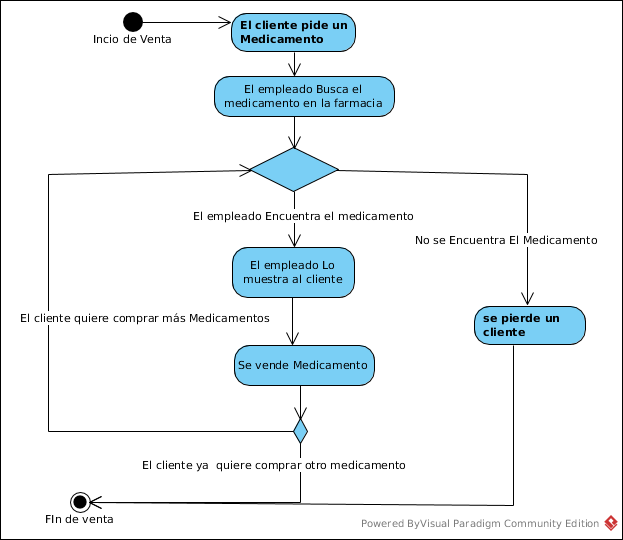
\includegraphics[width=.7\textwidth]{images/AS-TOprocVenta}
		\caption{PROC-01 Realización de una venta al cliente}
		\label{fig:proceso1}
	\end{center}
\end{figure}

\begin{description}
	\item[Descripción:] Ocurre cuando llega un cliente a la farmacia en busca de un medicamento que quiere comprar, el empleado de planta se tarda aproximadamente 7min en buscar un medicamento,una vez que este se encuentra se le muestra al cliente y se vende. 
	\item[Entradas:] \cdtEmpty
        \begin{itemize}
			\item Cliente
			\item Dinero
        \end{itemize}
	\item[Salidas:] \cdtEmpty
        \begin{itemize}
			\item Medicamento
        \end{itemize}	
    \item[Áreas de oportunidad:]la búsqueda del medicamento será mucho más rápida y eficiente, lo cual le ahorra tiempo al cliente y a la farmacia aparte de tener mejor guardados los datos de una venta.
\end{description}

% - - - - - - - - - - - - - - - - - - - - - - - - - - - - 
\subsection{PROC-02 Contratar a nuevo personal}

\begin{figure}[htbp]
	\begin{center}
		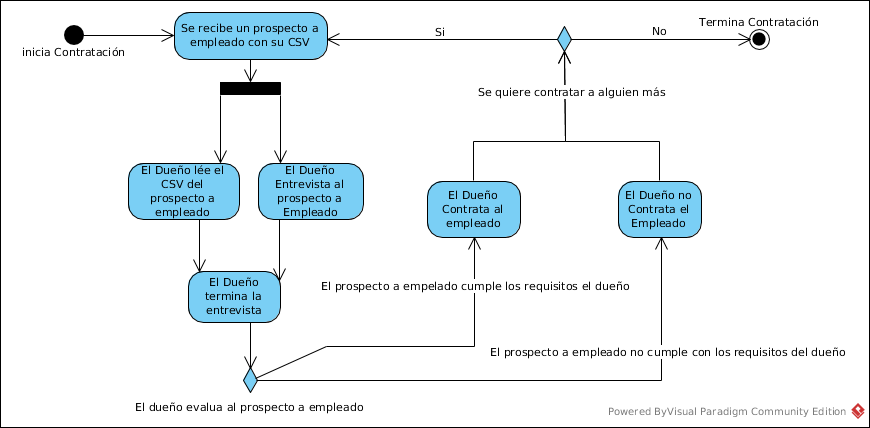
\includegraphics[width=.8\textwidth]{images/AS-toprocContratacion}
		\caption{PROC-02 Contratar a nuevo personal}
		\label{fig:proceso2}
	\end{center}
\end{figure}

\begin{description}
	\item[Descripción:] Cuando se abre una sucursal o simplemente hace falta personal, se procede a contratar a nuevo ya sea supervisor o solo empleado de planta. El Dueño es el que se encarga de la entrevista y de todo el proceso de la contratación.
	\item[Entradas:] \cdtEmpty
        \begin{itemize}
			\item Datos del prospecto a empleado
			\item Un nuevo empleado
        \end{itemize}
	\item[Salidas:] \cdtEmpty
        \begin{itemize}
			\item Contrato
        \end{itemize}	
    \item[Áreas de oportunidad:] Con el sistema funcionando, se facilitará la asignación de una sucursal a un empleado así como guardar los datos del empleado, y también ayudara al dueño a conocer y controlar de mejor forma a su personal.
\end{description}


% - - - - - - - - - - - - - - - - - - - - - - - - - - - - 
\subsection{PROC-03 Agregar medicamento del proveedor}

\begin{figure}[htbp]
	\begin{center}
		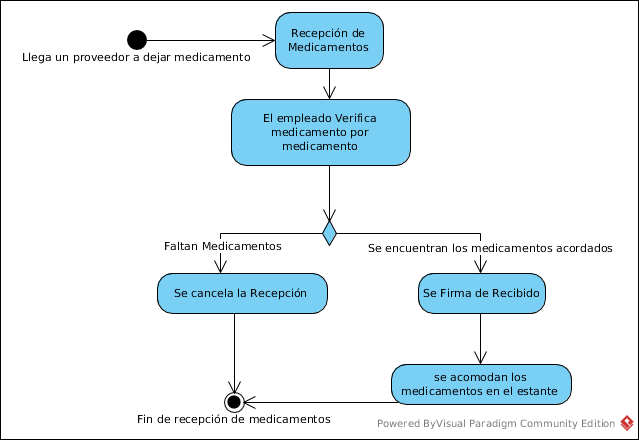
\includegraphics[width=.7\textwidth]{images/as-toprocAgreMedic}
		\caption{PROC-03 Agregar medicamento del proveedor}
		\label{fig:proceso1}
	\end{center}
\end{figure}

\begin{description}
	\item[Descripción:] Son Acciones realizadas por el empleado de planta en la farmacia, sucede cuando un proveedor trae una entrega, el empleado tiene que verificar que los medicamentos son los que se pidieron y procede a Firmar,pagar y acomodar los medicamentos en su  estante
	\item[Entradas:] \cdtEmpty
        \begin{itemize}
			\item Medicamentos.
			\item Nota de recibido.
        \end{itemize}
	\item[Salidas:] \cdtEmpty
        \begin{itemize}
			\item Dinero
			\item Medicamentos caducados
        \end{itemize}	
    \item[Áreas de oportunidad:] Con el sistema le sera más fácil controlar 
    El ingreso de medicamentos por un proveedor, si bien se tendrá que hacer un proceso más largo, este ayudara al empleado a entregar cuentas al supervisor de la sucursal.
     \end{description}

%---------------------------------------------------------
\section{Modelo de procesos TO-BE}

Los nuevos procesos se presentan en esta sección, el mapa de procesos de se muestra en la figura~\ref{fig:mapaProc}.

\begin{figure}[htbp]
	\begin{center}
		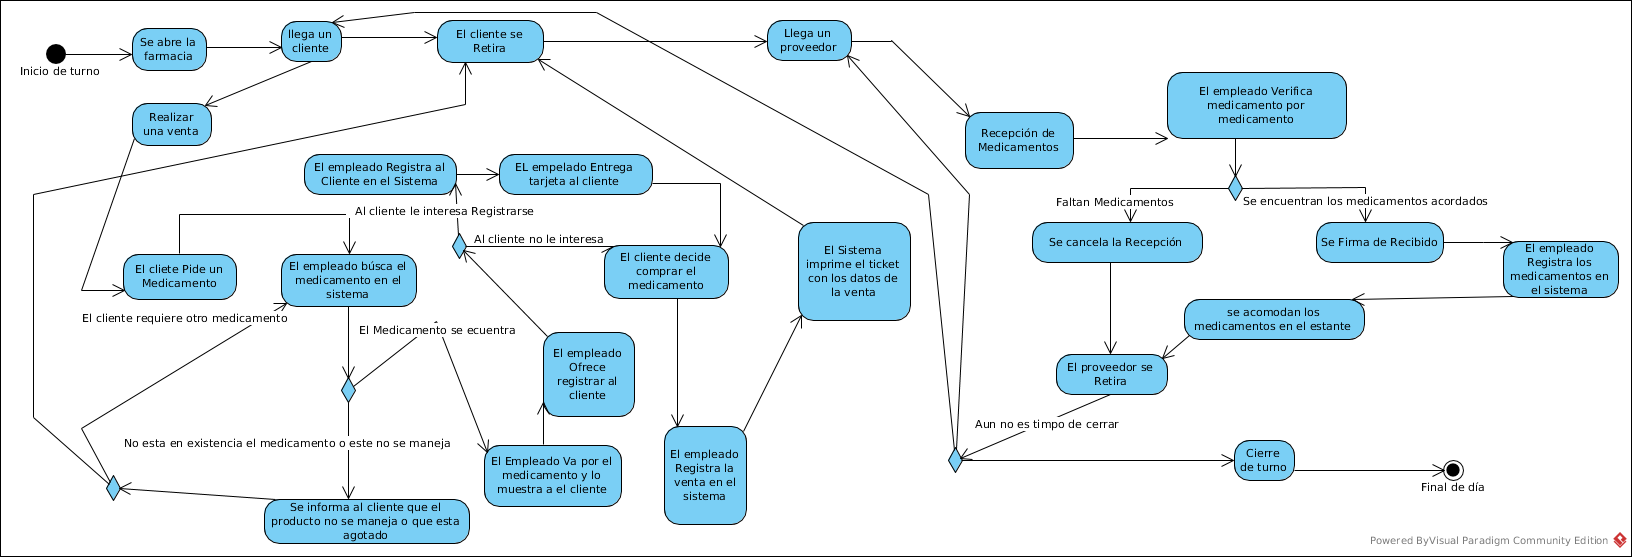
\includegraphics[width=.8\textwidth]{images/procMap}
		\caption{Mapa de procesos}
		\label{fig:mapaProc}
	\end{center}
\end{figure}

% - - - - - - - - - - - - - - - - - - - - - - - - - - - - 
\subsection{PROCM-01 Realizar una venta}

\begin{figure}[htbp]
	\begin{center}
		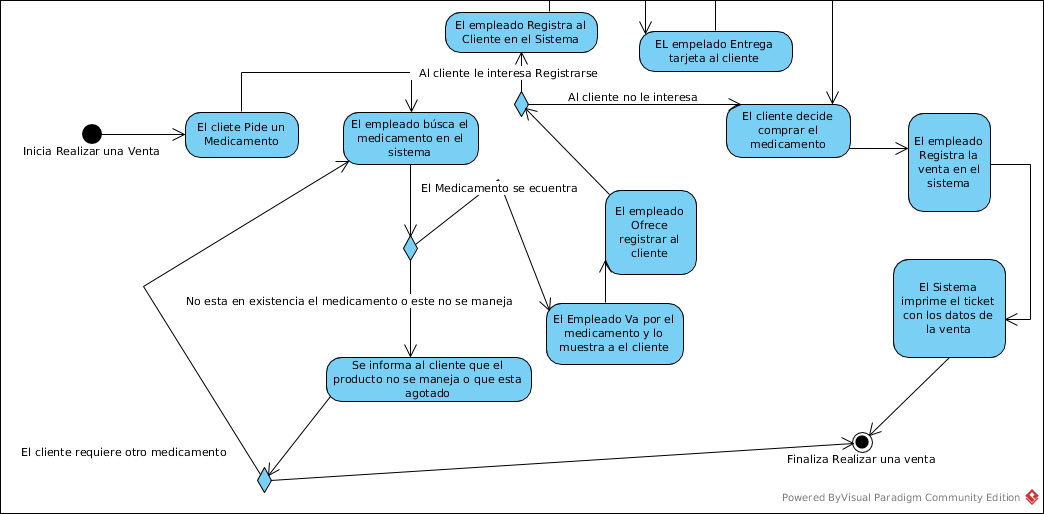
\includegraphics[width=.8\textwidth]{images/TOBERealizarVenta}
		\caption{PROCM-01 Realizar una venta}
		\label{fig:proceso3}
	\end{center}
\end{figure}

\begin{description}
	\item[Descripción:] Ahora con el sistema en función, cuando un cliente venga buscando un medicamento, se le podrá brindar de forma más rápida información de dicho medicamento.
	\item[Entradas:] \cdtEmpty
        \begin{itemize}
			\item nombre del medicamento
			\item ingredientes activos del medicamento.
			\item código de barras del medicamento.
        \end{itemize}
	\item[Salidas:] \cdtEmpty
        \begin{itemize}
			\item Datos del medicamento.
        \end{itemize}	
    \item[Mejoras esperadas:]se ahorra tiempo para la venta, lo cual le conviene al cliente y a la farmacia.
    \item[Casos de uso:] CU 39 Realizar una venta, CU 12 Listar medicamentos, CU33 Listar Clientes, CU 36 Registrar Clientes, CU35 Cambiar datos del cliente, CU 32 Hacer devolución al cliente, CU31 Darle crédito a un cliente, CU30 Aplcar credito de un cliente, CU29 Registrar una venta como devolución, CU25 Reporte de Ventas Por empleado.
\end{description}

% - - - - - - - - - - - - - - - - - - - - - - - - - - - - 
\subsection{PROCM-02 Contratar Nuevo Personal}

\begin{figure}[htbp]
	\begin{center}
		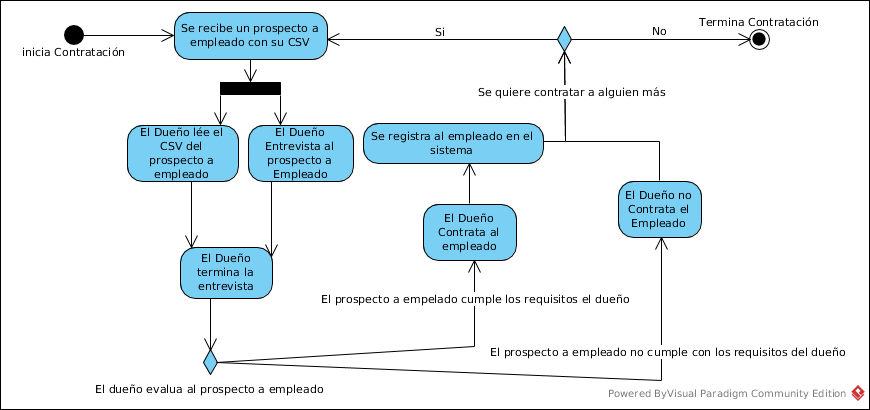
\includegraphics[width=.8\textwidth]{images/TOBEprocContratacion}
		\caption{PROCM-02 Contratar Nuevo Personal}
		\label{fig:proceso3}
	\end{center}
\end{figure}

\begin{description}
	\item[Descripción:]Cuando se abre una nueva sucursal o simplemente se esta escaso de personal, se procede a la contratación del nuevo, dicha contratación es llevada a cabo por el dueño, con el sistema en funcionamiento se espera que se tenga un mejor manejo de los nuevos empleados en la sucursal, así como facilitar la asignación del personal en una sucursal.
	\item[Entradas:] \cdtEmpty
        \begin{itemize}
			\item Datos del nuevo empleado
        \end{itemize}
	\item[Salidas:] \cdtEmpty
        \begin{itemize}
			\item Contrato
        \end{itemize}	
    \item[Mejoras esperadas:] se espera que ahora se pueda tener un mejor control de los empleados..
    \item[Casos de uso:]CU 8 Agregar Empleado.
\end{description}

% - - - - - - - - - - - - - - - - - - - - - - - - - - - - 
\subsection{PROCM-03 Registrar medicamento del proveedor}

\begin{figure}[htbp]
	\begin{center}
		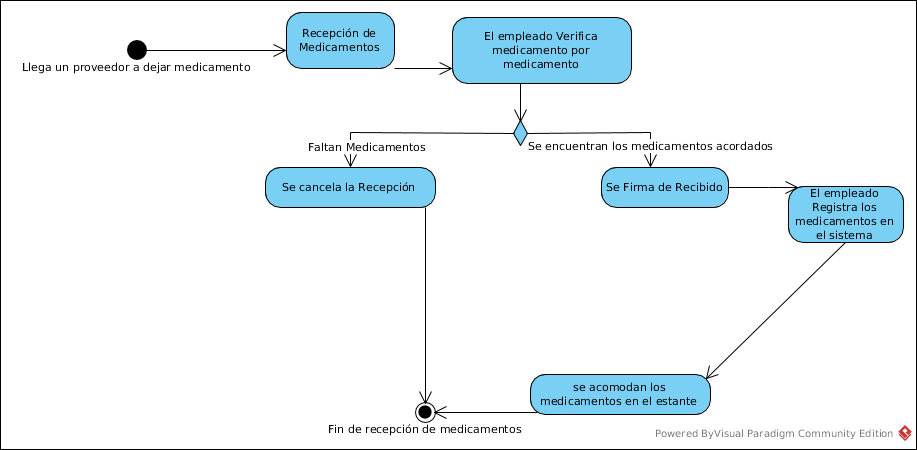
\includegraphics[width=.8\textwidth]{images/ToBEAgregarMedc}
		\caption{PROCM-03 Registrar medicamento del proveedor}
		\label{fig:proceso3}
	\end{center}
\end{figure}

\begin{description}
	\item[Descripción:] Cuando se llega un proveedor con un pedido de medicamento, 
	este se tiene que revisar y registrar en el sistema.
	\item[Entradas:] \cdtEmpty
        \begin{itemize}
			\item Datos del medicamento
        \end{itemize}
	\item[Salidas:] \cdtEmpty
        \begin{itemize}
			\item Dinero
        \end{itemize}	
    \item[Mejoras esperadas:] Este proceso es más lento que el anterior, pero ayuda a que existan menos incongruencias con los medicamentos en existencia, aparte de que ayuda a verificar de mejor forma los medicamentos que llegan del proveedor.
    \item[Casos de uso:] {CU 38 Registrar medicamentos del proveedor}, {CU 12 Listar medicamentos}.
\end{description}















